\chapter{Implementation of the method for unidirectional waves}

\section{Background}
The JONSWAP spectrum is defined as
\begin{subequations}
\begin{equation}
    S_{\eta \eta}(f) = \alpha H_s^2 f_p^4 f^{-5} \gamma^\beta \exp{\left[-\frac{5}{4}\left(\frac{f_p}{f}\right)^4\right]}
    \label{eq:JONSWAPSpec}
\end{equation} 
\begin{equation}
    \alpha =\frac{0.0624}{0.230+0.0336\gamma-\frac{0.185}{1.9+\gamma}} ,\quad \beta = \exp{\left[ -\frac{(f-f_p)^2}{2\sigma^2f_p^2} \right]}, \quad
    \sigma =
    \begin{cases}
    0.07, \quad \text{for }f\leq f_p \\
    0.09, \quad \text{for }f> f_p
    \end{cases}
    \label{eq:JONSWAPparam}
\end{equation}
\label{eq:JONSWAP}
\end{subequations}
where \cref{eq:JONSWAPSpec} defines the power spectrum and \cref{eq:JONSWAPparam} defines the suggested scalar parameters given in the slides. Here, $H_s$ is the significant wave height, $f_p$ is the frequency corresponding to the peak period (i.e. $f_p=1/T_p$), $f$ is the frequency of interest, $\gamma$ is the so-called peak enhancement factor and $\alpha$, $\beta$, $\sigma$ are scalar parameters describing the shape of the JONSWAP spectrum. 

The irregular wave series can be expressed using a Fourier series, where the standard Fourier representation can be written as
\begin{equation}
    \eta(t) = \sum_{n=1}^{n_{\text{max}}} a_n \cos{(\omega_n t)} +b_n \sin{(\omega_n t)}, \quad \text{where }\omega_n=\frac{2\pi}{T_n} \  \text{and} \ f_n=n\,df
\end{equation}
here $a_n$ and $b_n$ are the unknown Fourier coefficients, and $\omega_n$, $T_n$ and $f_n$ is the angular wave frequency, wave period, and wave frequency of each wave component, respectively. The equivalent complex representation can be formulated as
\begin{equation}
    \eta(t,x) = \sum_{n=1}^{n_{\text{max}}} c_n e^{-i(\omega_n t-k_n x)} + \Tilde{c}_n e^{i(\omega_n t - k_n x)}, \quad \text{where }c_n=\frac{1}{2}(a_n+i b_n) \ \text{and} \ \Tilde{c}_n=\frac{1}{2}(a_n-i b_n)
    \label{eq:ComplexFourier}
\end{equation}
which also shows the conversion between the real and complex Fourier coefficients. Note that the actual wave surface elevation is the real part of the above complex representation. Here the tilde $[\, \Tilde{\text{\scalebox{0.5}{\textbullet}}}\,]$ denotes the complex conjugate.

\begin{table}[h]
    \centering
    \caption{Model parameters (Group 10)}
    \begin{tabular}{@{}lllll@{}}
    \toprule
    Significance                            &   Symbol          & Unit       & Value \\ \hline
    Water depth                             &   $h$             & \si{m}     & 29   \\
    Significant wave height                 &   $H_{s}$         & \si{m}     & 6.75   \\
    Peak wave period                        &   $T_p$           & \si{s}     & 11.5  \\ \addlinespace[1mm]
    Peak enhancement factor                 &   $\gamma$        & \si{-}     & 3.0 \\ \addlinespace[1mm]
    Spreading factor                        &   $s$             & \si{-}     & 2.75   \\ \addlinespace[1mm]
    Duration of wave conditions             &   $t_{\text{dur}}$& \si{s}     & 3600   \\
    Time step size                          &   $dt$            & \si{s}     & 0.25   \\
    \bottomrule
    \end{tabular}
    \label{tab:Modelparameters}
\end{table}

\section{Implementation for unidirectional waves}

The first step in generating the wave time series is to compute the power spectrum, $S_{\eta \eta}(f)$, using the previously defined JONSWAP spectrum (\cref{eq:JONSWAP}). The JONSWAP spectrum is implemented into a MATLAB function denoted \verb+JONSWAP(Hs,fp,gam,fvec)+, which outputs the JONSWAP spectrum. The inputs are given (in order) as the significant wave height, the peak frequency, the peak enhancement factor and a vector containing the frequency discretization. The frequency discretization vector contains frequencies up to the Nyquist frequency, $f_{\text{Nyq}}(=\frac{1}{2dt})$, with the step size determined by the bandwidth of the frequency resolution, $df(=\frac{1}{t_{\text{dur}}})$, i.e. \verb+fvec+$=\{df\ 2df \ \dots \ f_{\text{Nyq}}\}^T$.

Having obtained the power spectrum up until the Nyquist frequency, the second step is to provide an estimate for the phase shift of each component, $\delta_n$. As this is phase angle cannot be determined from the spectrum, $S_{\eta \eta}(f)$, the usual procedure is to assume that $\delta_n$ is a uniformly distributed stochastic variable over the interval $0<\delta_n\leq 2\pi$. The uniform distribution is achieved using the MATLAB intrinsic (pseudo) random number generator \verb+rand()+, with a fixed seed for reproducibility (seed=100).

The third step is to determine the complex conjugate pair of Fourier coefficients $\{c_n,\ \Tilde{c_n}\}$. This is achieved by first determining the real Fourier coefficients using the relations
\begin{equation}
    A_n = \sqrt{2 S_{\eta \eta}(f_n)\,df}, \quad a_n=A_n\cos{(\delta_n)}, \quad b_n=A_n\sin{(\delta_n)}
\end{equation}
and then converting $\{a_n,\ b_n \}$ (using \cref{eq:ComplexFourier}) to the paired complex coefficients, $\{c_n,\ \Tilde{c}_n\}$.

The fourth step introduces a clever computational/theoretical trick, so it requires a short explanation. First, it is noticed that the  

\begin{figure}[htbp]
    \centering
    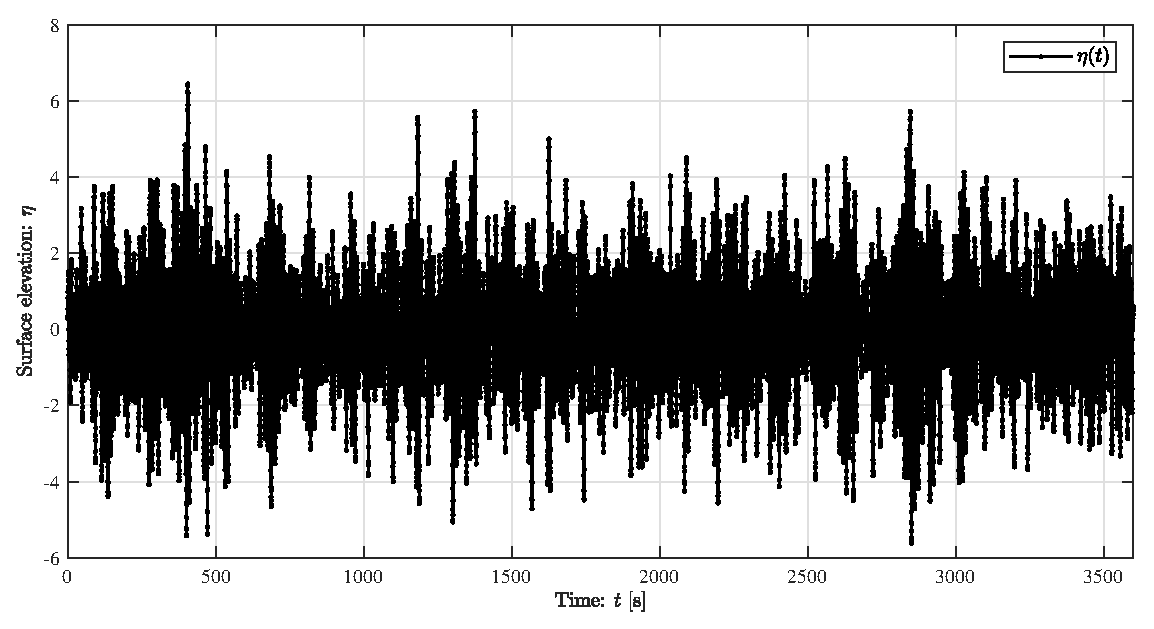
\includegraphics[width=0.9\textwidth]{Figures/Plots/SurfaceElevation.eps}
    \caption{Caption}
    \label{fig:my_label}
\end{figure}